\section{Auswertung}
\label{sec:Auswertung}
\subsection{Bestimmung der Brennweite über Linsengleichung.}
\label{sec:1}
Die gemessenen Werte  der Gegenstandsweite $g$ und der Bildweite $b$  sind
in der Tabelle \ref{tab:1} und \ref{tab:2} aufgeliste.
Die Linse der ersten Messung besitzt laut Herstellerangaben eine Brennweite $f$
von
\begin{align*}
  f_1=100\si{\milli\meter}\\
\intertext{und die der zweiten Linse eine von }
  f_2=150\si{\milli\meter}.
\end{align*}
Die gemessene Gegenstandsweiten und Bildweiten können nun in die Gleichung
\eqref{eqn:linse} eingesetzet werden um die entsprechende Brennweite $f$
zu erhalen. Ebenfalls ist in der Tabelle \ref{tab:1}
die Bildgröße enthalten somit lässt sich durch die Gegenstandsgröße, die
\begin{align*}
  G=30\si{\milli\meter}
\end{align*}
beträt, das Verhältnis zwischen $G/B$ und $g/b$ vergleichen. Dies ist ebenfalls
in der Tabelle \ref{tab:1} aufgelistet.
\begin{table}
  \centering
  \caption{Messwerte der 1. Messung und das aus der Gleichung
   \eqref{eqn:linse} berechnete $f$.}
  \label{tab:1}
  \begin{tabular}{c c c c c c}
  \toprule
  Gegenstandsweite   & Bildweite & Bildgröße & Brennweite & \multicolumn{2}{c}{Verhältniss}\\
  $g/\si{\milli\meter}$ & $b/\si{\milli\meter}$ & $B/\si{\milli\meter}$& $f/\si{\milli\meter}$& $G/B$ &$g/b$\\
  \midrule
  140   &   317  &   60 & 97 &0,5 &0,4 \\
  150   &   284  &   47 & 98 &0,6 &0,5 \\
  160   &   251  &   43 & 98 &0,7 &0,6 \\
  200   &   168  &   27 & 91 &1,1 &1,2 \\
  230   &   170  &   20 & 98 &1,5 &1,4 \\
  250   &   158  &   18 & 97 &1,7 &1,6 \\
  280   &   150  &   16 & 98 &1,9 &1,9 \\
  300   &   123  &   16 & 87 &1,9 &2,4 \\
  320   &   140  &   14 & 97 &2,1 &2,3 \\
  350   &   134  &   12 & 97 &2,5 &2,6 \\
  \bottomrule
 \end{tabular}
\end{table}
\FloatBarrier
\begin{table}
  \centering
  \caption{Messwerte der 2. Messung und das aus der Gleichung
   \eqref{eqn:linse} berechnete $f$.}
  \label{tab:2}
  \begin{tabular}{c c c}
  \toprule
  Gegenstandsweite   & Bildweite & Brennweite\\
  $g/\si{\milli\meter}$ & $b/\si{\milli\meter}$ & $f/\si{\milli\meter}$\\
  \midrule
  260  &  431 & 162\\
  250  &  480 & 164\\
  270  &  414 & 163\\
  280  &  395 & 164\\
  290  &  375 & 164\\
  300  &  357 & 163\\
  330  &  320 & 162\\
  350  &  306 & 163\\
  370  &  291 & 163\\
  400  &  275 & 163\\
  \bottomrule
\end{tabular}
\end{table}
\FloatBarrier
Werden die berechnenten Brennweiten $f$
nun gemittelt, ergibt sich für die erste Linse:
\begin{align*}
  f_{1_\mathrm{gemessen}}=(95,8\pm3,4)\si{\milli\meter}
\intertext{Für die zweite Linse:}
f_{2_\mathrm{gemessen}}=(163,2\pm0,6)\si{\milli\meter}
\end{align*}

Desweitern lassen sich die Genauigkeiten der Messwerte überprüfen,
indem die gemessene Gegenstandsweiten $g$ auf die x-Achse aufgetragen wird
und mit den entsprechenden Bildweiten $b$, die auf der y-Achse aufgertagen ist,
durch eine Linie verbunden wird. Die Abbildungen \ref{fig:1} und \ref{fig:2}
enthälten diese Methode.

\begin{figure}
 \centering
 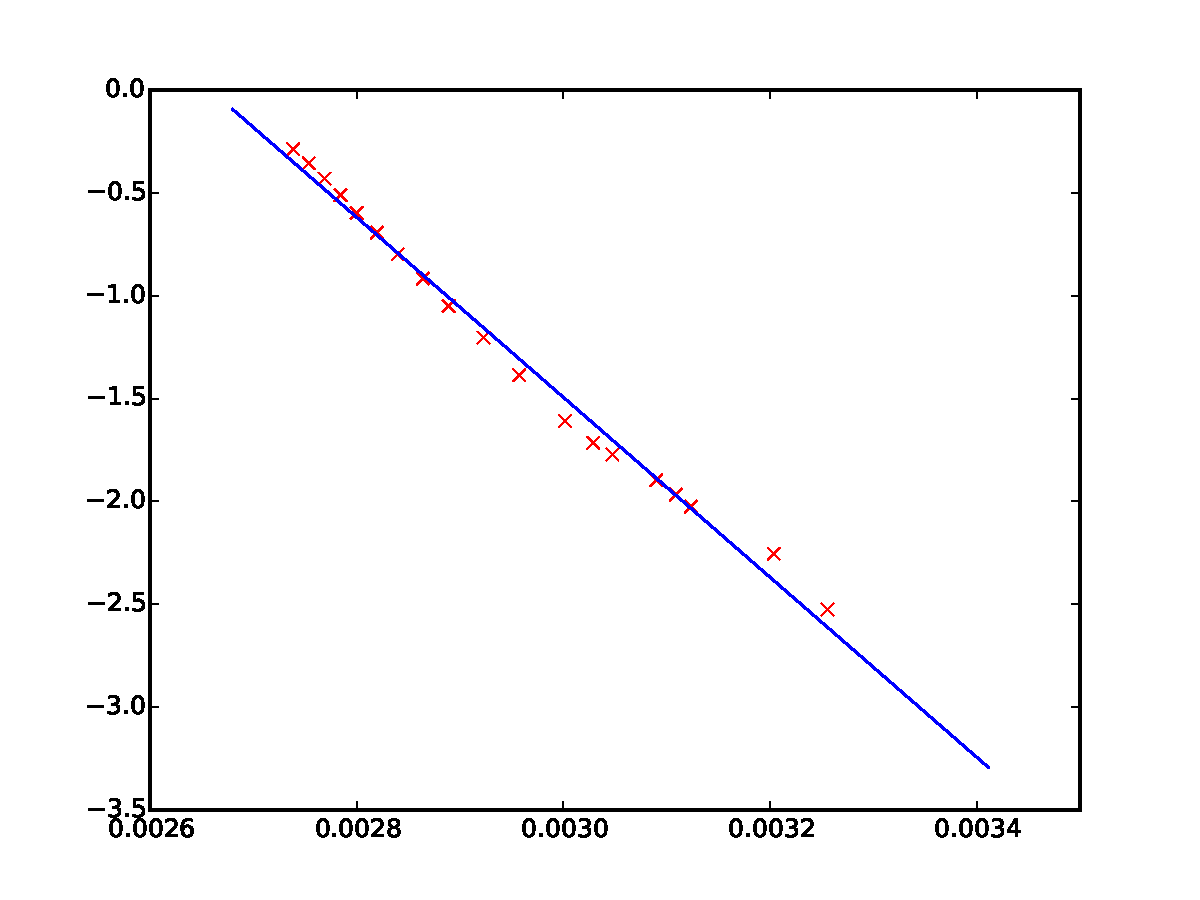
\includegraphics[width=0.7\textwidth]{plot1.pdf}
 \caption{Abblidung zur Bestimmung der Genauigkeit der 1. Messung}
 \label{fig:1}
\end{figure}
\FloatBarrier
\begin{figure}
 \centering
 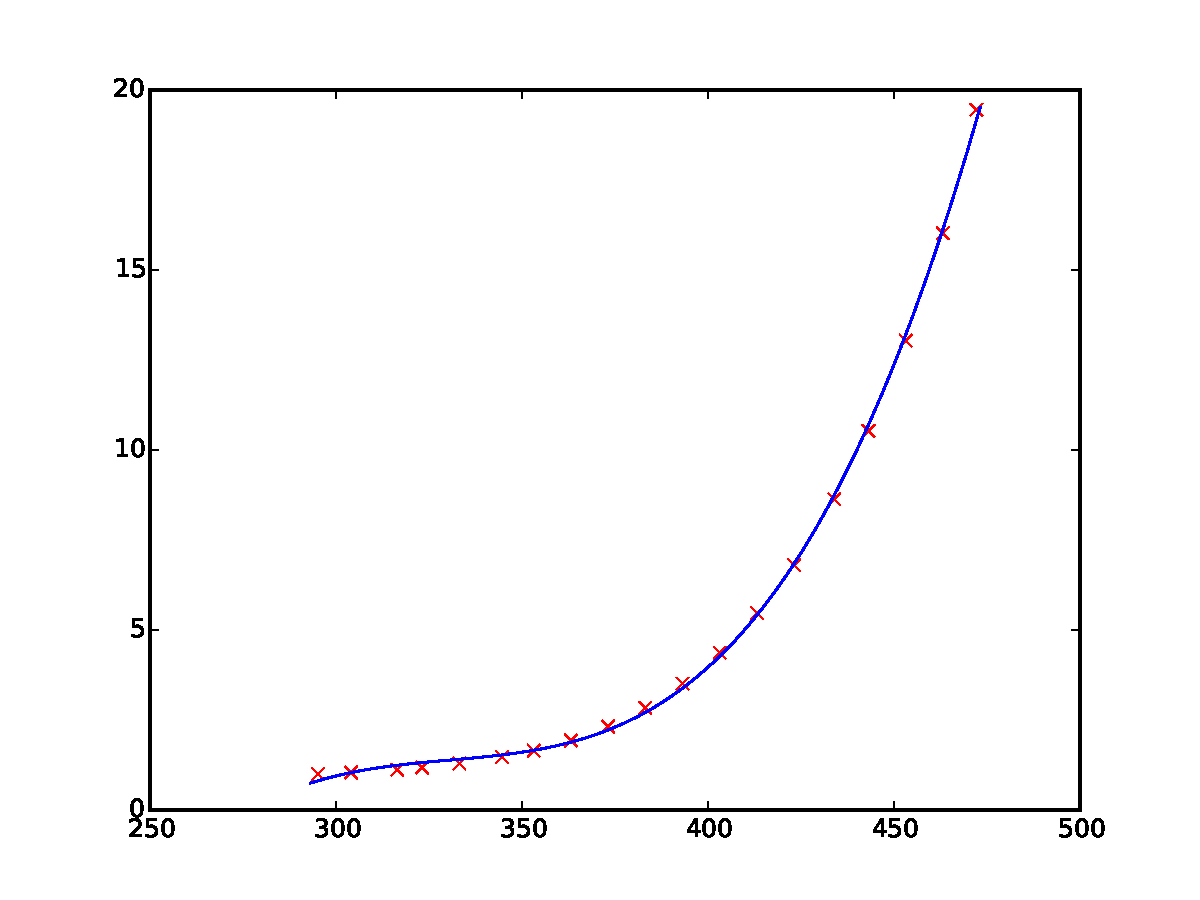
\includegraphics[width=0.7\textwidth]{plot2.pdf}
 \caption{Abblidung zur Bestimmung der Genauigkeit der 2. Messung}
 \label{fig:2}
\end{figure}
\FloatBarrier
\subsection{Bestimmung der Brennweite durch die Methode von Bessel.}
Die zuvermessene Linse besitzt lauf Herstellerangaben eine Brennweite von:
\begin{align*}
  f=150\si{\milli\meter}.
\end{align*}
Die Tabelle \ref{tab:bessel} enthält die Messwerte für die Messung mit der Bessel Methode.
Die Brennweite $f$ errechnet sich bei dieser Methode mit Hilfe der Formel \ref{eqn:bessel}.
\begin{table}
    \centering
    \caption{Messwerte die mit Hilfe der Methode von Bessel aufgenommen worden sind
    und die Brennweiten $f$ die über die Formel \eqref{eqn:Bessel} berechnet werden.}
    \label{tab:bessel}
    \begin{tabular}{c c c c c c c}
    \toprule
    Gegenstandsweite   & Bildweite &  Gegenstandsweite   & Bildweite & Abstand  & \multicolumn{2}{c}{Brennweite}\\
    $g_1/\si{\milli\meter}$ & $b_1/\si{\milli\meter}$ &$g_2/\si{\milli\meter}$ & $b_2/\si{\milli\meter}$ & e/\si{\milli\meter} & $f_1/\si{\milli\meter}$ & $f_2/\si{\milli\meter}$\\
    \midrule
  435  &   265 &   264 &   436  & 700  & 165 & 164 \\
  509  &   241 &   236 &   514  & 750  & 164 & 162 \\
  570  &   230 &   225 &   575  & 800  & 164 & 162 \\
  624  &   226 &   216 &   634  & 850  & 166 & 161 \\
  682  &   218 &   211 &   689  & 900  & 165 & 162 \\
  738  &   212 &   205 &   745  & 950  & 165 & 161 \\
  790  &   210 &   201 &   799  & 1000 & 166 & 161 \\
  842  &   208 &   198 &   852  & 1050 & 167 & 161 \\
  896  &   204 &   195 &   905  & 1100 & 166 & 160 \\
  950  &   200 &    95 &   1055 & 1150 & 165 & 87  \\
  \bottomrule
\end{tabular}
\end{table}
\FloatBarrier
Die Ergebnisse für die Brennweiten
werden wieder gemittelt und es ergibt sich ein $f$ von:
\begin{align*}
  f=(160\pm17)\si{\milli\meter}.
\end{align*}

Die Methode wird nun einmal mit einem  roten und einem blauen Filter durchgeführt.
Die Messwerte dafür sind für rot in der Tabelle \ref{tab:rot} und für blau
in der Tabelle \ref{tab:blau} gelistet.
Die Brennweiten $f$ berechnen sich wieder nach Formel \eqref{eqn:Bessel}.

\begin{table}
    \centering
    \caption{Messwerte die mit Hilfe der Methode von Bessel mit einem roten Filter aufgenommen worden sind.}
    \label{tab:rot}
    \begin{tabular}{c c c c c c c}
    \toprule
    Gegenstandsweite   & Bildweite &  Gegenstandsweite   & Bildweite & Abstand  & \multicolumn{2}{c}{Brennweite}\\
    $g_1/\si{\milli\meter}$ & $b_1/\si{\milli\meter}$ &$g_2/\si{\milli\meter}$ & $b_2/\si{\milli\meter}$ & e/\si{\milli\meter} & $f_1/\si{\milli\meter}$ & $f_2/\si{\milli\meter}$\\
    \midrule
    440 & 260 & 256 & 444 & 700  & 163  & 162 \\
    567 & 233 & 224 & 576 & 800  & 165  & 161 \\
    687 & 213 & 212 & 688 & 900  & 163  & 162 \\
    795 & 205 & 200 & 800 & 1000 & 163  & 160 \\
    907 & 193 & 193 & 907 & 1100 & 159  & 159 \\
    \bottomrule
\end{tabular}
\end{table}
\FloatBarrier

\begin{table}
    \centering
    \caption{Messwerte die mit Hilfe der Methode von Bessel mit einem blauen Filteraufgenommen worden sind.}
    \label{tab:blau}
    \begin{tabular}{c c c c c c c}
    \toprule
    Gegenstandsweite   & Bildweite &  Gegenstandsweite   & Bildweite & Abstand  & \multicolumn{2}{c}{Brennweite}\\
    $g_1/\si{\milli\meter}$ & $b_1/\si{\milli\meter}$ &$g_2/\si{\milli\meter}$ & $b_2/\si{\milli\meter}$ & e/\si{\milli\meter} & $f_1/\si{\milli\meter}$ & $f_2/\si{\milli\meter}$\\
    \midrule
    436  & 264  &  253  &  447  &  700  & 164 & 162 \\
    571  & 229  &  224  &  576  &  800  & 163 & 161 \\
    685  & 215  &  210  &  690  &  900  & 164 & 161 \\
    800  & 200  &  202  &  795  &  1000 & 160 & 162 \\
    905  & 195  &  195  &  905  &  1100 & 160 & 160 \\
    \bottomrule
  \end{tabular}
\end{table}
\FloatBarrier

Werden diese Ergebnisse nun gemittel, ergibt sich somit für
die Linse bei einem rotem Filter eine Brennweite von:
\begin{align*}
  f_\mathrm{rot}=(161,81\pm1,84)\si{\milli\meter}
\intertext{Für einem blauen Filter:}
  f_\mathrm{blau}=(161,83\pm1,45)\si{\milli\meter}
\end{align*}

\subsection{Bestimmung der Brennweite eines Linsensystems durch die Methode von Abbe.}
Das verwendete Linsensystem besteht hier
aus einer Zerstreuungslinse mit Brennweite
\begin{align*}
  f=-100\si{\milli\meter}
\intertext{und einer Sammellinse mit Brennweite}
  f=100\si{\milli\meter}
\intertext{die einen Abstand $d$ von}
  d=??\si{\milli\meter}
\end{align*}
zusammengeschoben sind.
Mit diesen Werten und der Formel \eqref{eqn:abbetheo} kann die theoretische
Brennweite $f_\mathrm{ges}$ des Linsensystems bestimmt werden.
\begin{align}
  \frac{1}{f_\mathrm{ges}}=\frac{1}{f_1}+\frac{1}{f_2}-\frac{d}{f_1f_2}\label{eqn:abbetheo}
\end{align}
Es ergibt sich ein Wert von:
\begin{align*}
  f_\mathrm{theo}=??
\end{align*}

In der Tabelle \ref{tab:abbe} sind die Messwerte der Messung nach der Methode von Abbe aufgeliste.
Der Abbildungsmaßstab $V$ wird aus der Formel \label{eqn:V} berechnet
\begin{align}
  V=\frac{B}{G}\label{eqn:V}
\end{align}


\begin{table}
    \centering
    \caption{Messwerte die mit Hilfe der Methode von Bessel mit einem blauen Filteraufgenommen worden sind.}
    \label{tab:blau}
    \begin{tabular}{c c c c c c c}
    \toprule
    Bildgröße  & Bildweite &Gegenstandsweite & Abbildungsmaßstab
     $B/\si{\milli\meter}$ &$b'/\si{\milli\meter}$ & $g'/\si{\milli\meter}$ &$V$\\
    \midrule
    32  &  528  &  272  & 1,07\\
    17  &  434  &  416  & 0,57\\
    16  &  412  &  488  & 0,53\\
    13  &  400  &  550  & 0,43\\
    12  &  395  &  606  & 0,40\\
    10  &  391  &  659  & 0,33\\
    9   &  377  &  723  & 0,3\\
    8   &  376  &  774  & 0,27\\
    8   &  368  &  832  & 0,27\\
    7   &  366  &  884  & 0,23\\
    \bottomrule
  \end{tabular}
\end{table}
\FloatBarrier
Um die Brennweite zu bestimmen, wird nun einmal
die Gegenstandweite $g'$ in Abhängigkeit von
%\begin{align*}
  $(1+ \frac{1}{V})$, wie in der  Abbildung \ref{fig:Plotg'} zu sehen,
sowie die Bildweite $b'$ in Abhängigkeit von
$(1+V)$ aufgetragen, siehe Abbildung\ref{fig:Plotb'}.


\begin{figure}
  \centering
  \includegraphics[width=0.7\textwidth]{plotabbeg.pdf}
  \caption{Die gemessene Gegenstandsweite $g'$ in Abhängigkeit von $1+\frac{1}{V}$.}
  \label{fig:Plotg'}
\end{figure}

\begin{figure}
 \centering
 \includegraphics[width=0.7\textwidth]{plotabbeb.pdf}
 \caption{Die gemessene Bildweite $b'$ in Abhängigkeit von $1+V$.}
 \label{fig:Plotb'}
\end{figure}
\FloatBarrier

Es wird nun eine lineare Ausgleichsrechnung mit den Messwerte durchgeführt.
Aus den Formeln  \eqref{eqn:abbeg} und \eqref{eqn:abbeb} und den Parameter der
Ausgleichsrechung ergeben sich die folgenden Werte:
\begin{align*}
\intertext{Aus der Gerade aus Abblidung \ref{fig:Plotg'} :}
  f_\mathrm{g'}=(181,6\pm7,7)\si{\milli\meter} \\
  h=(126,7\pm10,8)\si{\milli\meter} \\
\intertext{Aus der Gerade aus Abblidung \ref{fig:Plotb'} :}
f_\mathrm{b'}=(193,1\pm7,4)\si{\milli\meter} \\
  h'=(-60,5\pm29,9)\si{\milli\meter} \\
\end{align*}

Die beiden Ergebnisse der Brennweite $f$
werden nun gemittelt und es ergibt sich:
\begin{align*}
  f=(187\pm5)\si{\milli\meter}
\end{align*}
